\documentclass[floatsintext,doc]{apa6}
\usepackage{lmodern}
\usepackage{amssymb,amsmath}
\usepackage{ifxetex,ifluatex}
\usepackage{apacite}
%\usepackage{hyperref}

\usepackage{fixltx2e} % provides \textsubscript
\ifnum 0\ifxetex 1\fi\ifluatex 1\fi=0 % if pdftex
  \usepackage[T1]{fontenc}
  \usepackage[utf8]{inputenc}
\else % if luatex or xelatex
  \ifxetex
    \usepackage{mathspec}
  \else
    \usepackage{fontspec}
  \fi
  \defaultfontfeatures{Ligatures=TeX,Scale=MatchLowercase}
\fi
% use upquote if available, for straight quotes in verbatim environments
\IfFileExists{upquote.sty}{\usepackage{upquote}}{}
% use microtype if available
\IfFileExists{microtype.sty}{%
\usepackage{microtype}
\UseMicrotypeSet[protrusion]{basicmath} % disable protrusion for tt fonts
}{}

%\hypersetup{unicode=true,
%            pdftitle={Not unreasonable: Uncertainty in the language of logic},
%            pdfauthor={Michael Henry Tessler~\& Michael Franke},
%            pdfkeywords={semantics; pragmatics; negation; Bayesian cognitive model; Rational Speech Act},
%            pdfborder={0 0 0},
%            breaklinks=true}
%\urlstyle{same}  % don't use monospace font for urls
\usepackage{graphicx,grffile}
\makeatletter
\def\maxwidth{\ifdim\Gin@nat@width>\linewidth\linewidth\else\Gin@nat@width\fi}
\def\maxheight{\ifdim\Gin@nat@height>\textheight\textheight\else\Gin@nat@height\fi}
\makeatother
% Scale images if necessary, so that they will not overflow the page
% margins by default, and it is still possible to overwrite the defaults
% using explicit options in \includegraphics[width, height, ...]{}
\setkeys{Gin}{width=\maxwidth,height=\maxheight,keepaspectratio}
\IfFileExists{parskip.sty}{%
\usepackage{parskip}
}{% else
\setlength{\parindent}{0pt}
\setlength{\parskip}{6pt plus 2pt minus 1pt}
}
\setlength{\emergencystretch}{3em}  % prevent overfull lines
\providecommand{\tightlist}{%
  \setlength{\itemsep}{0pt}\setlength{\parskip}{0pt}}
\setcounter{secnumdepth}{0}
% Redefines (sub)paragraphs to behave more like sections
\ifx\paragraph\undefined\else
\let\oldparagraph\paragraph
\renewcommand{\paragraph}[1]{\oldparagraph{#1}\mbox{}}
\fi
\ifx\subparagraph\undefined\else
\let\oldsubparagraph\subparagraph
\renewcommand{\subparagraph}[1]{\oldsubparagraph{#1}\mbox{}}
\fi

%%% Use protect on footnotes to avoid problems with footnotes in titles
\let\rmarkdownfootnote\footnote%
\def\footnote{\protect\rmarkdownfootnote}


  \title{Not unreasonable: Uncertainty in the language of negation}
    \author{Michael Henry Tessler\textsuperscript{1}~\& Michael Franke\textsuperscript{2}}
    \date{}
  
\shorttitle{Uncertain logical language}
\affiliation{
\vspace{0.5cm}
\textsuperscript{1} Massachusetts Institute of Technology\\\textsuperscript{2} University of Osnabr\"{u}ck}
\keywords{semantics; pragmatics; negation; Bayesian cognitive model; Rational Speech Act\newline\indent Word count: X}
\usepackage{csquotes}
\usepackage{upgreek}
\captionsetup{font=singlespacing,justification=justified}

\usepackage{longtable}
\usepackage{lscape}
\usepackage{multirow}
\usepackage{tabularx}
\usepackage[flushleft]{threeparttable}
\usepackage{threeparttablex}

%\newenvironment{lltable}{\begin{landscape}\begin{center}\begin{ThreePartTable}}{\end{ThreePartTable}\end{center}\end{landscape}}

\makeatletter
\newcommand\LastLTentrywidth{1em}
\newlength\longtablewidth
\setlength{\longtablewidth}{1in}
\newcommand{\getlongtablewidth}{\begingroup \ifcsname LT@\roman{LT@tables}\endcsname \global\longtablewidth=0pt \renewcommand{\LT@entry}[2]{\global\advance\longtablewidth by ##2\relax\gdef\LastLTentrywidth{##2}}\@nameuse{LT@\roman{LT@tables}} \fi \endgroup}


%\DeclareDelayedFloatFlavor{ThreePartTable}{table}
%\DeclareDelayedFloatFlavor{lltable}{table}
%\DeclareDelayedFloatFlavor*{longtable}{table}
\makeatletter
%\renewcommand{\efloat@iwrite}[1]{\immediate\expandafter\protected@write\csname efloat@post#1\endcsname{}}
\makeatother
\usepackage{tabularx}
\usepackage{multicol}
\usepackage{wrapfig}
\usepackage{gensymb}
\usepackage{tikz}
\usepackage{caption}
\usepackage{booktabs}
\usepackage{xcolor}

\authornote{This work was supported in part by NSF Graduate Research Fellowship DGE-114747 to MHT.

Correspondence concerning this article should be addressed to Michael Henry Tessler, 43 Vassar St, Cambridge, MA 02139. E-mail: \url{tessler@mit.edu}}

\abstract{
Language provides multiple ways of conveying the opposite: A person \emph{not happy} can be \emph{unhappy}, \emph{sad}, or perhaps neither, just \emph{not happy}. Rather than being redundant, we hypothesize that uncertainty about the meaning of negation markers allows listeners to derive fine-grained distinctions among these various alternatives. We formalize this hypothesis in a probabilistic model of gradable adjectives (e.g., \emph{happy}), and use this to address an outstanding puzzle: how to interpret double negations (e.g., \emph{not unhappy}). Our model makes surprising additional predictions about a putative difference between morphological antonyms (\emph{unhappy}) and negated positives (\emph{not happy}): Listeners should judge \emph{unhappy} as more sad than \emph{not happy} only when confronted with alternatives in context; when interpreted in isolation, we predict no difference in understanding. Two behavioral experiments confirm consistent orderings of interpretations that interact with the presentational context in the way predicted. These findings support the hypothesis that listeners represent uncertainty even about the most logical elements of language.


}

\begin{document}
\maketitle

\newcommand*\diff{\mathop{}\!\mathrm{d}}
\newcommand{\denote}[1]{\mbox{ $[\![ #1 ]\!]$}}
\newcommand{\tableref}[1]{Table$\thinspace$\ref{#1}}
\newcommand{\figref}[1]{Fig.$\thinspace$\ref{#1}}
\newcommand{\appref}[1]{Appendix \ref{#1}}
\newcommand{\sectionref}[1]{Section \ref{#1}}
\definecolor{Red}{RGB}{255,0,0}
\definecolor{Green}{RGB}{10,200,100}
\definecolor{Blue}{RGB}{10,100,200}
\definecolor{grey}{RGB}{40,40,40}

\newcommand{\red}[1]{\textcolor{Red}{#1}}  
\newcommand{\mf}[1]{\textcolor{Green}{[mf: #1]}}  
\newcommand{\mht}[1]{\textcolor{Blue}{[mht: #1]}}

%\newcommand{\wrapmf}[1]{#1}

\providecommand{\tightlist}{%
  \setlength{\itemsep}{0pt}\setlength{\parskip}{0pt}}

\begin{quote}
Banal statements are given an appearance of profundity by means of the ``not un-'' formation. [$\ldots$] It should be possible to laugh the ``not un-'' formation out of existence by memorizing this sentence: ``A not unblack dog was chasing a not unsmall rabbit across a not ungreen field.'' 
\cite{orwell1946politics} (p.$\thinspace$357)
%(Orwell, 1946; )
\end{quote}

%\hypertarget{introduction}

In logic, two negatives make a positive.
With natural language, however, it is not always clear what should happen:
If \emph{Jones is not unhappy}, does that mean that Jones is happy?
\citeA{Jespersen1924} suggested not:

\begin{quote}
[T]wo negatives do not exactly cancel one another [$\ldots$]; the longer expression is always weaker: ``this is not unknown to me'' or ``I am not ignorant of this'' means ``I am to some extent aware of it,'' etc. (p.$\thinspace$332)
\end{quote}

In other words, \enquote{not unhappy} (a \emph{negated antonym}) could indicate a degree of happiness below that indicated by \enquote{happy} (a \emph{positive adjective}) but above those of \enquote{not happy} and \enquote{unhappy} (\emph{negated positives} and \emph{antonyms}, respectively; Fig.\(\thinspace\)\ref{fig:happy-scale}; \citeNP{Krifka2007:Negated-antonyms}).
This intuition is not uncontroversial---consider Orwell's quote above---nor is there agreement about how a listener derives a weakly positive interpretation from a double negative.
Antonyms created by morphology (\emph{morphological antonyms} e.g., \enquote{un}+\enquote{happy}) could convey a \emph{contrary} meaning, which is often conveyed by antonyms which have their own lexical entry (\emph{lexical antonyms} e.g., \enquote{sad}).
The key fact about contraries is that they can both be false (unlike logical \emph{contradictions}): Jones may be neither tall nor short (contraries) but a natural number cannot neither be even nor odd (contradictions; \citeNP{Horn1989:Natural}).
Pragmatically, \enquote{not unhappy} should compete with \enquote{happy} as an alternative description, resulting in a contextually strengthened interpretation corresponding to a neutral or indifferent state \cite{Horn1991:Duplex}, contra \citeA{Jespersen1924}'s intuition that \enquote{not unhappy} is a slightly positive state.
Such an analysis, however, further depends on the meaning of \enquote{not happy} (Blutner, 2004), of which there is also little agreement: \citeA{Jespersen1917:Negation} and \citeA{Blutner2004:pragmatics} believe that \enquote{not happy} means the same as \enquote{unhappy}, while \citeA{Krifka2007:Negated-antonyms} disagrees, citing examples like:

\begin{quote}
It's an absolutely horrible feeling to be unhappy, and I don't even think I was unhappy, just not happy, if you know what I mean. \emph{(taken from the internet)}
\end{quote}



How does such a logical linguistic device---negation---give rise to a multiplicity of meanings?
Both syntactic \cite{Cable2017} and pragmatic \cite{Rett2014:eval} mechanisms have been proposed, but heretofore there have been no computational accounts tested against human behavioral data.
In addition, what constitutes the ground truth has been left to the intuitions of trained theorists, who very often disagree what the meanings of these terms.
We hypothesize that \emph{lexical uncertainty}---uncertainty in the meaning of words---pervades even the language of logical devices, which interacts with conversational reasoning to give rise to a panoply of context-specific interpretations.
Specifically, we posit that overt negation markers (\enquote{not}, \enquote{un-}) can convey either contrary or contradictory opposition and that listeners resolve their uncertainty about the meaning in context.

\begin{figure}[h]
\centering 
\includegraphics{figs/happy-scale-1}  
\caption{Possible ordering of antonyms and their negations.}\label{fig:happy-scale}
\end{figure}

Formally, a gradable adjective (e.g., \enquote{happy}) is thought to be literally true if the degree associated with that adjective \(x\) (e.g., the degree of happiness) is greater than some contextually-determined threshold \(\theta_1\): \(\mbox{ $[\![ happy ]\!]$}(x, \theta): x > \theta_1\) \cite{Kennedy2007}.
If a negation marker (e.g., \enquote{not}) creates a contradictory statement, then the resulting meaning would simply be that the degree is less than or equal to the threshold: \(\neg \mbox{ $[\![ happy ]\!]$}(x, \theta_1): x \leq \theta_1\).
Alternatively, negation could create a \emph{contrary} meaning, where a new predicate is formed and which is assigned its own threshold \(\theta_2\): \(\mbox{ $[\![ \tilde{happy} ]\!]$}(x, \theta_2): x < \theta_2\).
\mht{i think this point could be moved to a model implementation appendix or footnote}
\red{Contradictory opposition can be iterated (\(\neg \neg Hx\)) but contrary opposition cannot \cite{Horn1989:Natural}.
As a result, a single negative (\enquote{not happy} and \enquote{unhappy}) can mean either \(\neg happy\) or \(\tilde{happy}\), while double negatives (\enquote{not unhappy}) may mean \(\neg \neg happy\) or \(\neg \tilde{happy}\) (Fig.\(\thinspace\)\ref{fig:lexicon-model}).}

In order to generate predictions, we formalize this \emph{uncertain negation} hypothesis in a probabilistic model of pragmatic reasoning in the Rational Speech Act tradition \cite{Franke2015a, Goodman2016:RSA}, a recursive reasoning model wherein a pragmatic listener \(L_{1}\) tries to resolve the intended meaning of an utterance \(u\) (e.g., \enquote{Jones is not unhappy}) by combining its prior beliefs about the degree of Jones' happiness \(P(x)\) with the Gricean assumption that speakers are generally cooperative \(S_1\) (Eqs.\(\thinspace\)\ref{eq:L1}-\ref{eq:L0}):
Listener uncertainty about the interpretation of negation markers is modeled as uncertainty about the speaker's lexicon \(\mathcal{L}\) \cite{Bergen2016}.
We combine this technique with the model of \citeA{Lassiter2015} that derives thresholds \(\theta\) for interpreting vague adjectives (e.g., happy) in context:

\vspace*{-0.5cm}

\begin{align}
L_{1}(x, \theta, \mathcal{L} \mid u) &\propto S_{1}(u \mid x, \theta, \mathcal{L}) \cdot P(x) \cdot  P(\theta) \cdot P(\mathcal{L}) \label{eq:L1} \\
S_{1}(u \mid x, \theta, \mathcal{L}) &\propto \exp{(\alpha \cdot \ln {L_{0}(x \mid u, \theta, \mathcal{L})} - \text{cost}(u))} \label{eq:S1}\\
L_{0}(x \mid u, \theta, \mathcal{L}) &\propto \mathcal{L}(u, x, \theta) \cdot P(x) \label{eq:L0}
\end{align}

The speaker model \(S_1\) (Eq.\ref{eq:S1}) describes an approximately rational agent (with degree of rationality \(\alpha\)) trying to inform a naive listener \(L_0\) about the degree \(x\).
The literal listener \(L_0\) (Eq. \ref{eq:L0}) updates its prior beliefs \(P(x)\) via an utterance's literal meaning in lexicon \(\mathcal{L}\),
where \(\mathcal{L}(u, x, \theta)\) gives the truth-value of \(u\) in lexicon \(\mathcal{L}\) applied to state \(x\) under threshold \(\theta\) (e.g., for $u= $\enquote{happy}, determining whether or not \(x>\theta\)).
The pragmatic listener (Eq. \ref{eq:L1}) has uncertainty about \(\theta\), which comes from an uninformed prior \(P(\theta)\) (following \citeNP{Lassiter2015}) and is resolved by jointly reasoning about the likely degree \(P(x)\), the likely lexicon \(P(\mathcal{L})\), and the likelihood \(S_1(u \mid x, \theta, \mathcal{L})\) that a cooperative information-maximizing speaker would utter the adjective given a degree \(x\), threshold \(\theta\), and lexicon \(\mathcal{L}\).

\begin{figure}
\centering
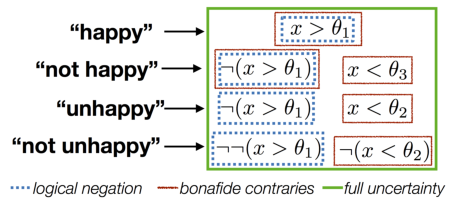
\includegraphics{figs/lexicon-model-1.pdf}
\caption{\label{fig:lexicon-model}Space of possible meanings in the lexicon prior for the \emph{logical negation}, \emph{bonafide contraries}, and the full \emph{uncertain negation} models.}
\end{figure}

We compare the predictions of this uncertain negation model to three theoretically-interesting alternative models.
First, we compare to a vanilla RSA model which has neither uncertainty about negation nor vagueness about the meaning of the adjective \cite{Frank2012}.\footnote{
The vanilla model assumes fixed-thresholds to the adjectives, and we assume antonyms convey contrary meanings. Therefore, we ascribe the following meanings to the adjectives: \enquote{happy} means \(>70\%\) on the happiness scale; \enquote{unhappy} means \(<30\%\).
}
Second, we compare to the vague RSA model of \citeA{Lassiter2015}, assuming that all negation marker entail contradictory negation (the \emph{logical negation} or \emph{George Orwell} model).
Finally, we construct a \emph{bonafide antonyms} model, building on \citeA{Lassiter2015}'s vague RSA model but where morphological antonyms (\emph{un-}) convey contrary negation.

%{]}
%--\textgreater{}

Upon hearing \enquote{not unhappy}, our \emph{uncertain negation} model reasons that a truly compositional \(\neg \neg \textit{happy}\) is implausible because the speaker could have just said the simpler \enquote{happy.}\footnote{Model predictions use the following minimally assumptive model parameters: \(P(x) = \mathcal{N}(0, 1); \alpha = 1; \text{cost}(\mathit{un}) = 1 < \text{cost}(\mathit{not}) = 2\).
  Predictions are qualitatively similar when \(\text{cost}(\mathit{un}) = \text{cost}(\mathit{not})\).}
interprets the utterance as signaling a slightly positive state (Fig.\(\thinspace\)\ref{fig:modelPredictions})
At the same time, the uncertain negation model does not differentiate \enquote{unhappy} (antonyms) from \enquote{not happy} (negated positives), as \citeA{Jespersen1917:Negation} and \citeA{Blutner2004:pragmatics} surmised.

The model draws these inferences by reasoning about which lexicon best explains a speaker's single utterance (Fig.\(\thinspace\)\ref{fig:modelPredictions}, \emph{single utterance}).
Hearing multiple utterances by the same speaker, however, can provide the listener more information about the speaker's lexicon, via a mutual-exclusitivity type effect.
The formal modeling approach we take hear naturally allows for this extension by conditioning \(L_1\) on the observation of a speaker using multiple adjective alternatives to describe different referents (e.g., \enquote{John is not happy. Bill is unhappy}; Fig.\(\thinspace\)\ref{fig:modelPredictions}, \emph{multiple utterances}).
When the model hears multiple utterances in the same context, the model does indeed predict a meaning difference between \enquote{unhappy} and \enquote{not happy}: \enquote{unhappy} is more sad than \enquote{not happy}, producing the ordering hypothesized by \citeA{Krifka2007:Negated-antonyms} in Fig.\ref{fig:happy-scale}.

This pattern of judgments is uniquely predicted by the \emph{uncertain negation} model.
The \emph{bonafide contraries} models also yields interpretations of negated antonyms as slightly positive, but predicts Krifka's ordering for both single and multiple utterance conditioning.
The \emph{logical negation} class does not differentiate between negated antonyms and positives, nor between negated positives and antonyms.
All models have more extreme interpretations when they condition on multiple utterances.

\section{Overview of Experiments}

The \emph{uncertain negation model} predicts a partial ordering for morphological antonyms and their negations when heard in isolation (with antonyms \(\approx\) negated positives), but a full ordering when present in the same context (Fig.\(\thinspace\)\ref{fig:modelPredictions}).
As a control condition, we examine antonyms which do not have overt negation markers (e.g., \emph{short}).
These lexical antonyms should behave like \emph{bonafide antonyms}, which predicts a full ordering regardless of context.
\text{Expt.$\thinspace$1} was exploratory and informed our computational modeling.
\text{Expt.$\thinspace$2} is a larger, more stringent, preregistered (\url{osf.io/p7f25/}) replication.
Finally, \text{Expt.$\thinspace$3} asks how specific the patterns of inferences are to morphological negation (\emph{un-}) as opposed to negation more broadly. 

%\hypertarget{behavioral-experiments}



\begin{figure}[t]
\centering 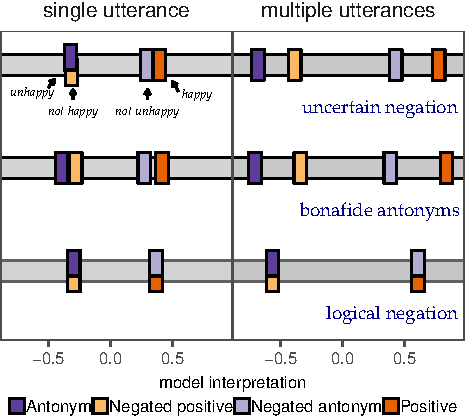
\includegraphics{figs/modelPredictions-1} 
\caption{ \emph{Uncertain negation} listener model (Eq.1) posterior expectations on a normalized scale (x-axis) for different adjective types (color). The space of possible meanings is restricted for \emph{bonafide antonyms} and \emph{logical negation} simulations (Fig.2). Paddles are vertically-offset when overlapping.}\label{fig:modelPredictions}
\end{figure}

%\hypertarget{experiment-1-single-utterances}{%
%\subsection{Experiment 1: Single utterances}\label{experiment-1-single-utterances}
%}

\subsection{Methods}
%\hypertarget{participants}

We recruited 120 participants from Amazon's Mechanical Turk (MTurk).
This number was arrived at with the intention of getting approximately 25 ratings for each unique item in the experiment.
In all experiments, participants were restricted to those with U.S. IP addresses and at least a 95\% work approval rating; in addition, participants who self-reported a native language other than English were excluded.
The experiment took on average 3 minutes and participants were compensated \$0.40.

%\hypertarget{procedure}

On each trial, participants read a statement introducing a person using a gradable adjective of one of four \emph{adjective types}: positives (e.g., \emph{happy}, \emph{tall}), antonyms (e.g., \emph{short}, \emph{unhappy}), and their respective negations (\emph{not} X).
Antonyms were one of two types: morphological (e.g., \emph{unhappy}) and lexical (e.g., \emph{short}).
Participants rated the character on a scale from \enquote{the most \emph{positive} person} to \enquote{the most \emph{antonym} person} (item-dependent) using a slider bar (Fig.$\thinspace$\ref{fig:experiment-slides}A).
Participants rated one sentence at a time and saw items from both antonym types throughout the experiment.
Each participant completed a total of 16 trials, with exactly 2 repetitions of each adjective type for each antonym type.

%\hypertarget{materials}

We used adjectives that described properties of people.
We refer to a collection of the four associated adjective forms---positives, antonyms (morphological or lexical), and their negations using the particle \enquote{not}---that have the same positive adjective as an \emph{adjective set} (e.g., one adjective set is \emph{happy}, \emph{unhappy}, \emph{not happy}, \emph{not unhappy}).
10 adjective sets were constructed for each antonym type (total 20) from an informal survey of the linguistics literature and taken from a list of \enquote{common opposites} available online (Table 1).\footnote{\url{http://www.enchantedlearning.com/wordlist/opposites.shtml}}
Each trial of the experiment used an adjective from a distinct adjective set (e.g., if a participant rated \emph{unhappy}, they rated no other adjective from the \{\emph{happy}, \emph{unhappy}, \ldots{}\} set).

\begin{table}[h]
\centering
\begingroup\fontsize{10pt}{11pt}\selectfont
\begin{tabular}{ll}
  \hline
Morphological antonyms & Lexical antonyms \\ 
  \hline
attractive, unattractive & beautiful, ugly \\ 
  educated, uneducated & brave, cowardly \\ 
  friendly, unfriendly & fat, skinny \\ 
  happy, unhappy & hard-working, lazy \\ 
  honest, dishonest & loud, quiet \\ 
  intelligent, unintelligent & proud, humble \\ 
  interesting, uninteresting & rich, poor \\ 
  mature, immature & strong, weak \\ 
  polite, impolite & tall, short \\ 
  successful, unsuccessful & wise, foolish \\ 
   \hline
\end{tabular}
\endgroup
\caption{Items in Experiment 1.} 
\end{table}

%\hypertarget{results}

6 participants were excluded for self-reporting a native language other than English, leaving a remainder of 114 participants for these analyses, which resulted in on average 23 ratings for each unique adjective in our stimulus set.
The qualitative predictions of our models concern the ordering within a set of alternatives for different antonym types (morphological vs.~lexical).
%To visualize the data, we compute normalized responses on a participant-wise basis (i.e., normalized response \(r'_{ij} = \frac{r_{ij} - mean_j}{sd_j}\) for trial \(i\) and participant \(j\)).
\red{Fig.$\thinspace$\ref{fig:expt-results}A shows the empirical distributions for each of the four adjective types for both morphological and lexical antonyms adjective sets.}
Critically, as predicted by the uncertain negation model, adjective sets with morphological antonyms show only a partial ordering, while those with lexical antonyms show a full ordering.

To confirm these observations, we built a linear mixed model predicting the raw, unnormalized ratings in terms of fixed effects of \emph{antonym type} (morphological vs.~lexical), \emph{adjective type} (Helmert coded in order: antonym, negated positive, negated antonym, positive)\footnote{Throughout, we code adjective type using Helmert coding, which compares levels of a factor to the average of preceding levels, in order to compare antonym vs.~negated positive levels of the adjective type factor.}, and their interaction; the model also included random intercepts and random slopes of \emph{adjective type} by-participant and by-item.\footnote{This, and all subsequent regression models, were the maximal mixed-effects model that converged for the data set that additionally explained significantly more variance than models with simpler mixed-effects structures, using the \texttt{lme4} package in R \cite{lme4}.}
Consistent with our observations, the difference between the \emph{antonym} vs. \emph{negated positive} levels of adjective type interacted significantly with antonym type (morphological vs.\text{~}lexical; \(\beta = 0.03\), t\((16) = 2.40, p = 0.03\)).

We also observe that negated morphological antonyms (e.g., \emph{not unhappy}) were rated lower than negated lexical antonyms (e.g., \emph{not tall}; Fig.$\thinspace$\ref{fig:expt-results}A).
Closer investigation of responses revealed that negated antonyms (and not other adjective types) received a bimodal distribution: Most ratings were slightly positive but a clearly distinguishable minority distribution of ratings were slightly negative (e.g., \emph{not dishonest} meaning \emph{not honest}).
This weakly negative interpretation for negated antonyms was present at least somewhat in every item and in most participants.
This interpretation may be the result of participants attributing politeness to the speaker: \emph{Not dishonest} may be an indirect way of saying that a person is not honest (Yoon, Tessler, Goodman, \& Frank, 2017).

\begin{figure}[hbt]

{\centering 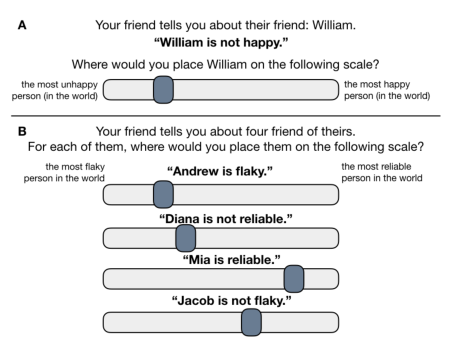
\includegraphics{figs/experiment-slides-1} 

}

\caption{Example experimental trials for (A) single utterance (Expts. 1, 2) and (B) multiple utterances conditions (Expt. 2). ``in the world'' wording for endpoints was used in Expt. 2. (A) shows a trial from a morphological antonym set while (B) shows a lexical antonym set.}\label{fig:experiment-slides}
\end{figure}

\begin{figure*}[h]
\centering 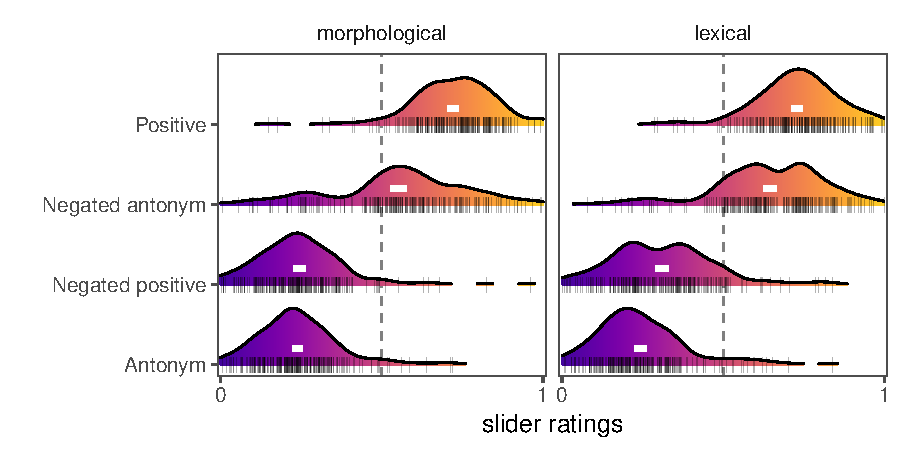
\includegraphics[width=0.95\linewidth]{figs/expt1_ridges_wCIs} 
\caption{Experiment 1 results. Empirical distributions of responses for adjective sets with morphological antonyms (e.g., ``unhappy'') and lexical antonyms (e.g., ``sad''). Dashed line indicates the midpoint of the scale. Dashes below density plots denote individual responses. White bars denote bootstrapped 95\% confidence intervals.}\label{fig:expt1-results}
\end{figure*}

%\hypertarget{experiment-2-single-and-multiple-utterances}

\text{Expt.$\thinspace$1} revealed an asymmetry: Lexical antonyms (e.g., \emph{short}) were clearly distinguished from negated positives (e.g., \emph{not tall}), whereas morphological antonyms were not (e.g., \emph{unhappy} \(\approx\) \emph{not happy}).
In \text{Expt.$\thinspace$1}, our adjective sets varied both in terms of their antonym type (morphological vs.\text{~}lexical) as well as the actual degree scales being described (e.g., height for \emph{tall}/\emph{short} vs.\text{~}happiness for \emph{happy}/\emph{unhappy}).
Many adjective sets have both morphological and lexical antonyms (e.g., \emph{happy}/\emph{unhappy}/\emph{sad}).
Here, we aim to replicate the asymmetry findings using adjectives that describe the same semantic scales.
Also, we test our second prediction that hearing multiple utterances in the same context will produce the full ordering for morphological antonym sets (Fig.\(\thinspace\)\ref{fig:modelPredictions}).

\subsection{Methods}
%\hypertarget{participants-1}

We recruited 750 participants from MTurk.
The experiment comprised of four between-subjects experimental conditions arranged in a 2x2 design: \emph{antonym type (morphological vs.\text{~}lexical)} X \emph{context (single vs.\text{~}multiple utterances)}.
300 participants were assigned to each \emph{antonym type} in the \emph{single utterance} contexts, and 75 participants were assigned to each in the \emph{multiple utterances} conditions.
These numbers follow from the intention of getting approximately 45 ratings for each unique adjective in the experiment.
The \emph{single utterance} task took on average 3 minutes and participants were compensated \$0.40; \emph{multiple utterances} took on average 5 minutes and participants were compensated \$0.80.
Exclusion criterion, sample size, procedure, and the analysis described below were preregistered: \url{osf.io/p7f25/}.

%\hypertarget{materials-1}

To best isolate the contribution of morphological vs.\text{~}lexical antonyms, we curated adjective sets consisting of words for properties of people, such that both types of antonyms existed for the same positive adjective (e.g., \emph{happy} \(\rightarrow\) \emph{unhappy}, \emph{sad}; \text{Table$\thinspace$2}).
Lexical antonyms were selected from a set of possibilities produced from a small survey (n=18) on MTurk eliciting \enquote{opposites} for a list of 30 positive-form adjectives which had morphological antonyms (asking participants in the same experimental context as our interpretation studies, \enquote{What is the opposite of e.g., \emph{forgiving}?}).
From the list of freely-produced opposites (the vast majority of which were not morphological), the first author chose the one that intuitively best conveyed the same scalar dimension as the morphological antonym and which was not already used as a lexical antonym for another item (e.g., opposite of \emph{forgiving} \(\rightarrow\) \emph{resentful}; opposite of \emph{kind} \(\rightarrow\) \emph{cruel}, because opposite of \emph{friendly} \(\rightarrow\) \emph{mean}).
Ten out of the original 30 items were dropped for either not having such a well-suited lexical antonym (e.g., \emph{moral}) or for having a well-suited lexical antonym that conflicted with another item (e.g., \emph{compassionate} \(\rightarrow\) \emph{cold}, but also \emph{affectionate} \(\rightarrow\) \emph{cold}).

%\hypertarget{procedure-1}

In the \emph{multiple utterances} conditions, participants rated all four adjective types simultaneously, each referring to a different person (Fig.$\thinspace$\ref{fig:experiment-slides}B), for a total of 12 trials.
The \emph{single utterances} conditions were similar to that of \text{Expt.$\thinspace$1}: Participants rated one sentence at a time (e.g., \enquote{Greg is not unhappy}), each from a unique adjective set (e.g., never rated both \emph{unhappy} and \emph{not happy}), completing a total of 12 trials, with exactly 3 repetitions of each adjective type (positive, antonym, and their negations).
In contrast to \text{Expt.$\thinspace$1}, \emph{antonym type} (morphological vs.\text{~}lexical) was a between-participants factor.
In addition, the slider bar endpoints were relabeled to \enquote{the most \{\emph{positive}, \emph{negative}\} person \emph{in the world}}; without \enquote{in the world}, there is a salient interpretation of the endpoints indicating \enquote{the most \{\emph{positive}, \emph{negative}\} person (of these four)} in the multiple utterances conditions.

\begin{table}[h]
\centering
\begingroup\fontsize{9pt}{10pt}\selectfont
\begin{tabular}{lll}
  \hline
Positive adjective & Morphological antonym & Lexical antonym \\ 
  \hline
affectionate & unaffectionate & cold \\ 
  ambitious & unambitious & lazy \\ 
  attractive & unattractive & ugly \\ 
  educated & uneducated & ignorant \\ 
  forgiving & unforgiving & resentful \\ 
  friendly & unfriendly & mean \\ 
  generous & ungenerous & stingy \\ 
  happy & unhappy & sad \\ 
  honest & dishonest & deceitful \\ 
  intelligent & unintelligent & stupid \\ 
  interesting & uninteresting & boring \\ 
  kind & unkind & cruel \\ 
  mature & immature & childish \\ 
  patriotic & unpatriotic & traitorous \\ 
  polite & impolite & rude \\ 
  rational & irrational & crazy \\ 
  reliable & unreliable & flaky \\ 
  resourceful & unresourceful & wasteful \\ 
  sincere & insincere & fake \\ 
  tolerant & intolerant & bigoted \\ 
   \hline
\end{tabular}
\endgroup
\caption{Items used in Experiment 2.} 
\end{table}

%\hypertarget{results-1}

35 participants were excluded for self-reporting a native language other than English, leaving 715 participants for these analyses.
Mean normalized responses for each adjective type in each condition are shown in Fig.$\thinspace$\ref{fig:expt-results}B.

As we did in \text{Expt.$\thinspace$1}, we evaluate our hypothesis that morphological antonyms behave like the \emph{uncertain negation} model (i.e., show a partial ordering) while lexical antonyms show a true ordering (like \emph{bonafide contraries}).
We considered data only from the \emph{single utterances} conditions and built a linear mixed model predicting the unnormalized ratings in terms of \emph{antonym type} (morphological vs.\text{~}lexical), \emph{adjective type} (Helmert coded in order: antonym, negated positive, negated antonym, positive) and their interaction; the model also included random intercepts and random slopes of \emph{adjective type} by-participant and by-item.
Consistent with our hypothesis, the interaction between the \emph{antonym} vs.\text{~}\emph{negated positive} levels of adjective type and antonym type (morphological vs.\text{~}lexical) was significant (\(\beta = 0.01\), t\((565) = 2.68, p = 0.01\)).
We then analyzed the simple effects.
Morphological antonyms were not significantly different than negated positives (\(\beta = 5.3e-05\), t\((52) = 0.02, p = 0.98\)), while lexical antonyms were interpreted more negatively than negated positives (\(\beta = -0.01\), t\((280) = 3.66\),
\(p = 0.00\)).\footnote{The random effect structure for the simple effects models mirrored the full model. The only difference was that in analyzing the lexical antonyms, the random effect of adjective type by-item needed to be dropped in order for the model to converge.}

Our second main hypothesis is that context (single vs.\text{~}multiple utterances) modulates the interpretive difference between morphological antonyms and negated positives.
Specifically, we predict that morphological antonyms will be interpreted more negatively than negated positives in a context with multiple utterances.
To evaluate this hypothesis, we considered data only from the morphological antonyms conditions and built a linear mixed model predicting the raw, unnormalized ratings in terms of adjective type,
context (single vs.~multiple utterances) and their interaction; the model also included random intercepts and random slopes of adjective type by-participant and by-item.
This interaction was also significant (\(\beta = 0.03\), t\((6457) = 6.73, p = 1.9e-11\)), and in the correct direction (see Fig.\text{~}\ref{fig:expt-results}B).
As an exploratory analysis, we examined these effects in a full three-way interactive model.
The relevant \emph{antonym} vs. \emph{negated positive} by adjective type (lexical, morphological) by context three-way interaction was in the direction of lexical antonyms showing a larger \emph{antonym} vs. \emph{negated positive} difference in the explicit context, but it was not significant (\(\beta = 0.01\), t\((469) = 1.64, p = 0.1\)).

%\hypertarget{discussion}

\mht{other thoughts: (a) dimensionality in antonyms (unhappy and sad map onto slightly different dimensions); (b) how much of this is specific to (American) English? [there is an oft intuition that Orwell believes this because he is british]; (c) relation to understatement more broadly}

Many dimensional scales lack units.
Speakers cannot say they are \emph{42 units happy} like they can say they are \emph{6'1" tall}.
Instead, speakers can use modifiers and morphemes to carve more precise meanings from otherwise vague dimensions.
A person \emph{not unhappy} is neither sad nor truly happy, but residing in some marginally positive state that is difficult to refer to because degrees of happiness lack precise units.

This work provides a computational solution to an outstanding puzzle in natural language understanding: How to interpret double negatives (e.g., \emph{not unhappy}; Krifka, 2007; Rett, 2014).
We additionally discovered and confirmed a surprising empirical result that challenges ``established'' intuitions in linguistics: \emph{unhappy} and \emph{not happy} are not immediately differentiated, except when both are present in the same context.
Our model that represents uncertainty about how to interpret overt negation markers (\emph{un-}, \emph{not}) predicts this very result, while alternative models that treat negation with a fixed meaning fall short.
One limitation of this work is that we stipulate, rather than derive, differences in meaning for morphological vs.~lexical antonym pairs (cf., Rett, 2014).

It is noteworthy that we are able to recover, both in our model and empirically, the ordering predicted by Krifka (2007) for morphological antonyms when a listener hears multiple adjectival utterances in the same context (\emph{multiple utterances condition}).
This work thus carries with it an account of a robust linguistic intuition: Potentially equivalent expressions receive differential interpretations when observed uttered by the same speaker in close proximity.
Reasoning about lexical ambiguity, listeners conclude that a choice of different expressions may be most likely for a speaker who differentiates meanings.
More generally, the inferences modeled here can be seen as an instance of \emph{mutual exclusivity} (Markman, 1989), in which listeners resolve uncertainty about multiple elements of meaning simultaneously.

Our formalization of lexical uncertainty about the meaning of natural language negation builds on a growing movement to treat the combinatorial rules of grammar as not totally separable from the lexicon (e.g., Bybee, 2006; O'Donnell, 2015).
Recent psycholinguistic evidence supports the idea that utterances which are heavily used will be processed as unique lexical entries while less frequent phrases will be understood compositionally (Morgan \& Levy, 2016).
The two types of negation meaning we considered---contrary and contradictory opposition---can be seen as a \emph{lexicalized} form of opposition (with the adjective receiving its own threshold variable) and a \emph{compositional} rule (logical negation), respectively.
In our modeling, we assumed all lexica (all logically-possible interpretations of negation) were equally likely \emph{a priori}: A further test of our negation uncertainty model would be to see if frequency can serve as a proxy for this prior over lexica.

To negate is to make true false, but for statements that are truly vague, the behavior of negation is not so obvious.
We present a computational explanation for why this is so, and provide empirical data that sheds new light on the age old question of meaning and opposition.

\newpage

%\hypertarget{references}{%
%\section{References}\label{references}%}



\bibliographystyle{apacite}

\setlength{\bibleftmargin}{.125in}
\setlength{\bibindent}{-\bibleftmargin}

\bibliography{negant}
%
%\begingroup
%\setlength{\parindent}{-0.5in}
%\setlength{\leftskip}{0.5in}
%
%\hypertarget{refs}{}
%\leavevmode\hypertarget{ref-lme4}{}%
%Bates, D., M\wrapmf{\"{a}}chler, M., Bolker, B., \& Walker, S. (2015). Fitting linear mixed-effects models using lme4. \emph{Journal of Statistical Software}, \emph{67}(1), 1--48.
%
%\leavevmode\hypertarget{ref-Bergen2016}{}%
%Bergen, L., Levy, R., \& Goodman, N. D. (2016). Pragmatic reasoning through semantic inference. \emph{Semantics and Pragmatics}, \emph{9}.
%
%\leavevmode\hypertarget{ref-Blutner2004:pragmatics}{}%
%Blutner, R. (2004). Pragmatics and the lexicon. \emph{Handbook of Pragmatics}, \emph{488514}.
%
%\leavevmode\hypertarget{ref-bybee2006usage}{}%
%Bybee, J. L. (2006). From usage to grammar: The mind's response to repetition. \emph{Language}, \emph{82}(4), 711--733.
%
%\leavevmode\hypertarget{ref-Cable2017}{}%
%Cable, S. (2017). The good, the 'not good', and the 'not pretty': Negation in the negative predicates of tlingit.
%
%\leavevmode\hypertarget{ref-Franke2015a}{}%
%Franke, M., \& J\wrapmf{\"{a}}ger, G. (2015). Probabilistic pragmatics, or why Bayes' rule is probably important for pragmatics. In \emph{Zeitschrift für sprachwissenschaft} (pp. 3--44).
%
%\leavevmode\hypertarget{ref-Goodman2016:RSA}{}%
%Goodman, N. D., \& Frank, M. C. (2016). Pragmatic language interpretation as probabilistic inference. \emph{Trends in Cognitive Sciences}, \emph{20}(11), 818--829.
%
%\leavevmode\hypertarget{ref-Horn1989:Natural}{}%
%Horn, L. R. (1989). \emph{A natural history of negation}. University of Chicago Press.
%
%\leavevmode\hypertarget{ref-Horn1991:Duplex}{}%
%Horn, L. R. (1991). Duplex negatio affirmat...: the economy of double negation. \emph{CLS 27-II: Papers from the Parasession on Negation}, 80--106.
%
%\leavevmode\hypertarget{ref-Jespersen1917:Negation}{}%
%Jespersen, O. (1917). \emph{Negation in english and other languages}. Kobenhavn: Host.
%
%\leavevmode\hypertarget{ref-Jespersen1924}{}%
%Jespersen, O. (1924). \emph{The philosophy of grammar}. London: Allen \& Unwin.
%
%\leavevmode\hypertarget{ref-Kennedy2007}{}%
%Kennedy, C. (2007). Vagueness and grammar: the semantics of relative and absolute gradable adjectives. \emph{Linguistics and Philosophy}, \emph{30}, 1--35.
%
%\leavevmode\hypertarget{ref-Krifka2007:Negated-antonyms}{}%
%Krifka, M. (2007). Negated Antonyms: Creating and Filling the Gap. \emph{Presupposition and Implicature in Compositional Semantics}, 163--177.
%
%\leavevmode\hypertarget{ref-Lassiter2015}{}%
%Lassiter, D., \& Goodman, N. D. (2015). Adjectival vagueness in a Bayesian model of interpretation. \emph{Synthese}.
%
%\leavevmode\hypertarget{ref-Markman1989}{}%
%Markman, E. M. (1989). \emph{Categorization and naming in children: Problems of induction}. MIT Press.
%
%\leavevmode\hypertarget{ref-MorganLevy2016:binomials}{}%
%Morgan, E., \& Levy, R. (2016). Abstract knowledge versus direct experience in processing of binomial expressions. \emph{Cognition}, \emph{157}, 384--402.
%
%\leavevmode\hypertarget{ref-Odonnell2015productivity}{}%
%O'Donnell, T. J. (2015). \emph{Productivity and reuse in language: A theory of linguistic computation and storage}. MIT Press.
%
%\leavevmode\hypertarget{ref-Rett2014:eval}{}%
%Rett, J. (2014). \emph{The semantics of evaluativity}. Oxford University Press.
%
%\leavevmode\hypertarget{ref-Yoon2017}{}%
%Yoon, E. J., Tessler, M. H., Goodman, N. D., \& Frank, M. C. (2017). "I won't lie, it wasn't amazing": Modeling polite indirect speech. In \emph{Proceedings of the 39th annual meeting of the cognitive science society}.
%
%\endgroup


\end{document}
